% \documentclass{standalone}
% \usepackage{currfile,hyperxmp}

% \input{../tikz_header.tex}

% \begin{document}



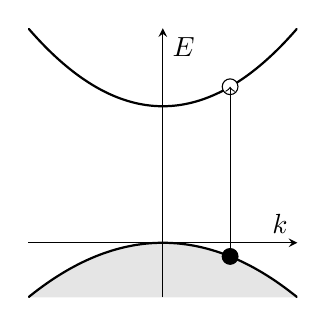
\begin{tikzpicture}
%\useasboundingbox (-1.3,-1.2) rectangle (10.2,4.7);
%\draw (-1,-1) rectangle +(12,5);

    \begin{axis}[ xlabel={ $k$}, ylabel= {$E$}, 
         width=50mm, height=50mm, 
        %ymode=log, 
     %   ymode=log,
      %   xmin = 0,
      %  xmax = 55,
    %     xmax = 4.4,
      %   ymin  = 0,
      %   ymax = 8,
         %xmax=5.5, ymin = 0, ymax=7.5,
         axis x line=center,
         axis y line=center,
         % xmax= 2e5, unbounded coords=jump, ymin=0, ymax = 4
        % label style={font=\tiny},
        % tick label style={font=\tiny}
        ytick= \empty ,
        xtick= \empty, 
     %  legend pos= north west,
     %  legend style={draw=none, font=\footnotesize}
    %clip = false,
    axis on top,
    ]

    %\fill[fill=gray!20!white] (0,0) rectangle (3,7);



 
    \addplot[thick,  domain=-2:2, samples = 100] {7 + x^2};
    \addplot[thick,  fill=gray!20!white, domain=-2:2, samples = 100] {- 0.7 * x^2};

    \coordinate (el) at (1, 8);
    \coordinate (hole) at (1, -0.7);
      

  
% \addplot[ mark=o, mark size = 1pt,  thick
% ] table [ col sep=comma,  
% x index = 0,
%  y expr = (\thisrowno{1} -10)  ,
% ] {\currfiledir data/MnO_Strauser_Wollan_80K.csv};

    %\draw[dashed] (1,-0.02) -- (1, 2.);   
    \node[right] at (15.3, 7) {$\omega_P$}; 
    \node[] at (8, 5.5) {$\omega_{SP}$}; 



    \end{axis}

    \draw[fill=white] (el) circle (0.1);
    \draw[fill=black] (hole) circle (0.1);
    \draw[<-] (el) -- (hole);

\end{tikzpicture}

%\end{document}